\begin{figure*}[!t]
    \centering
    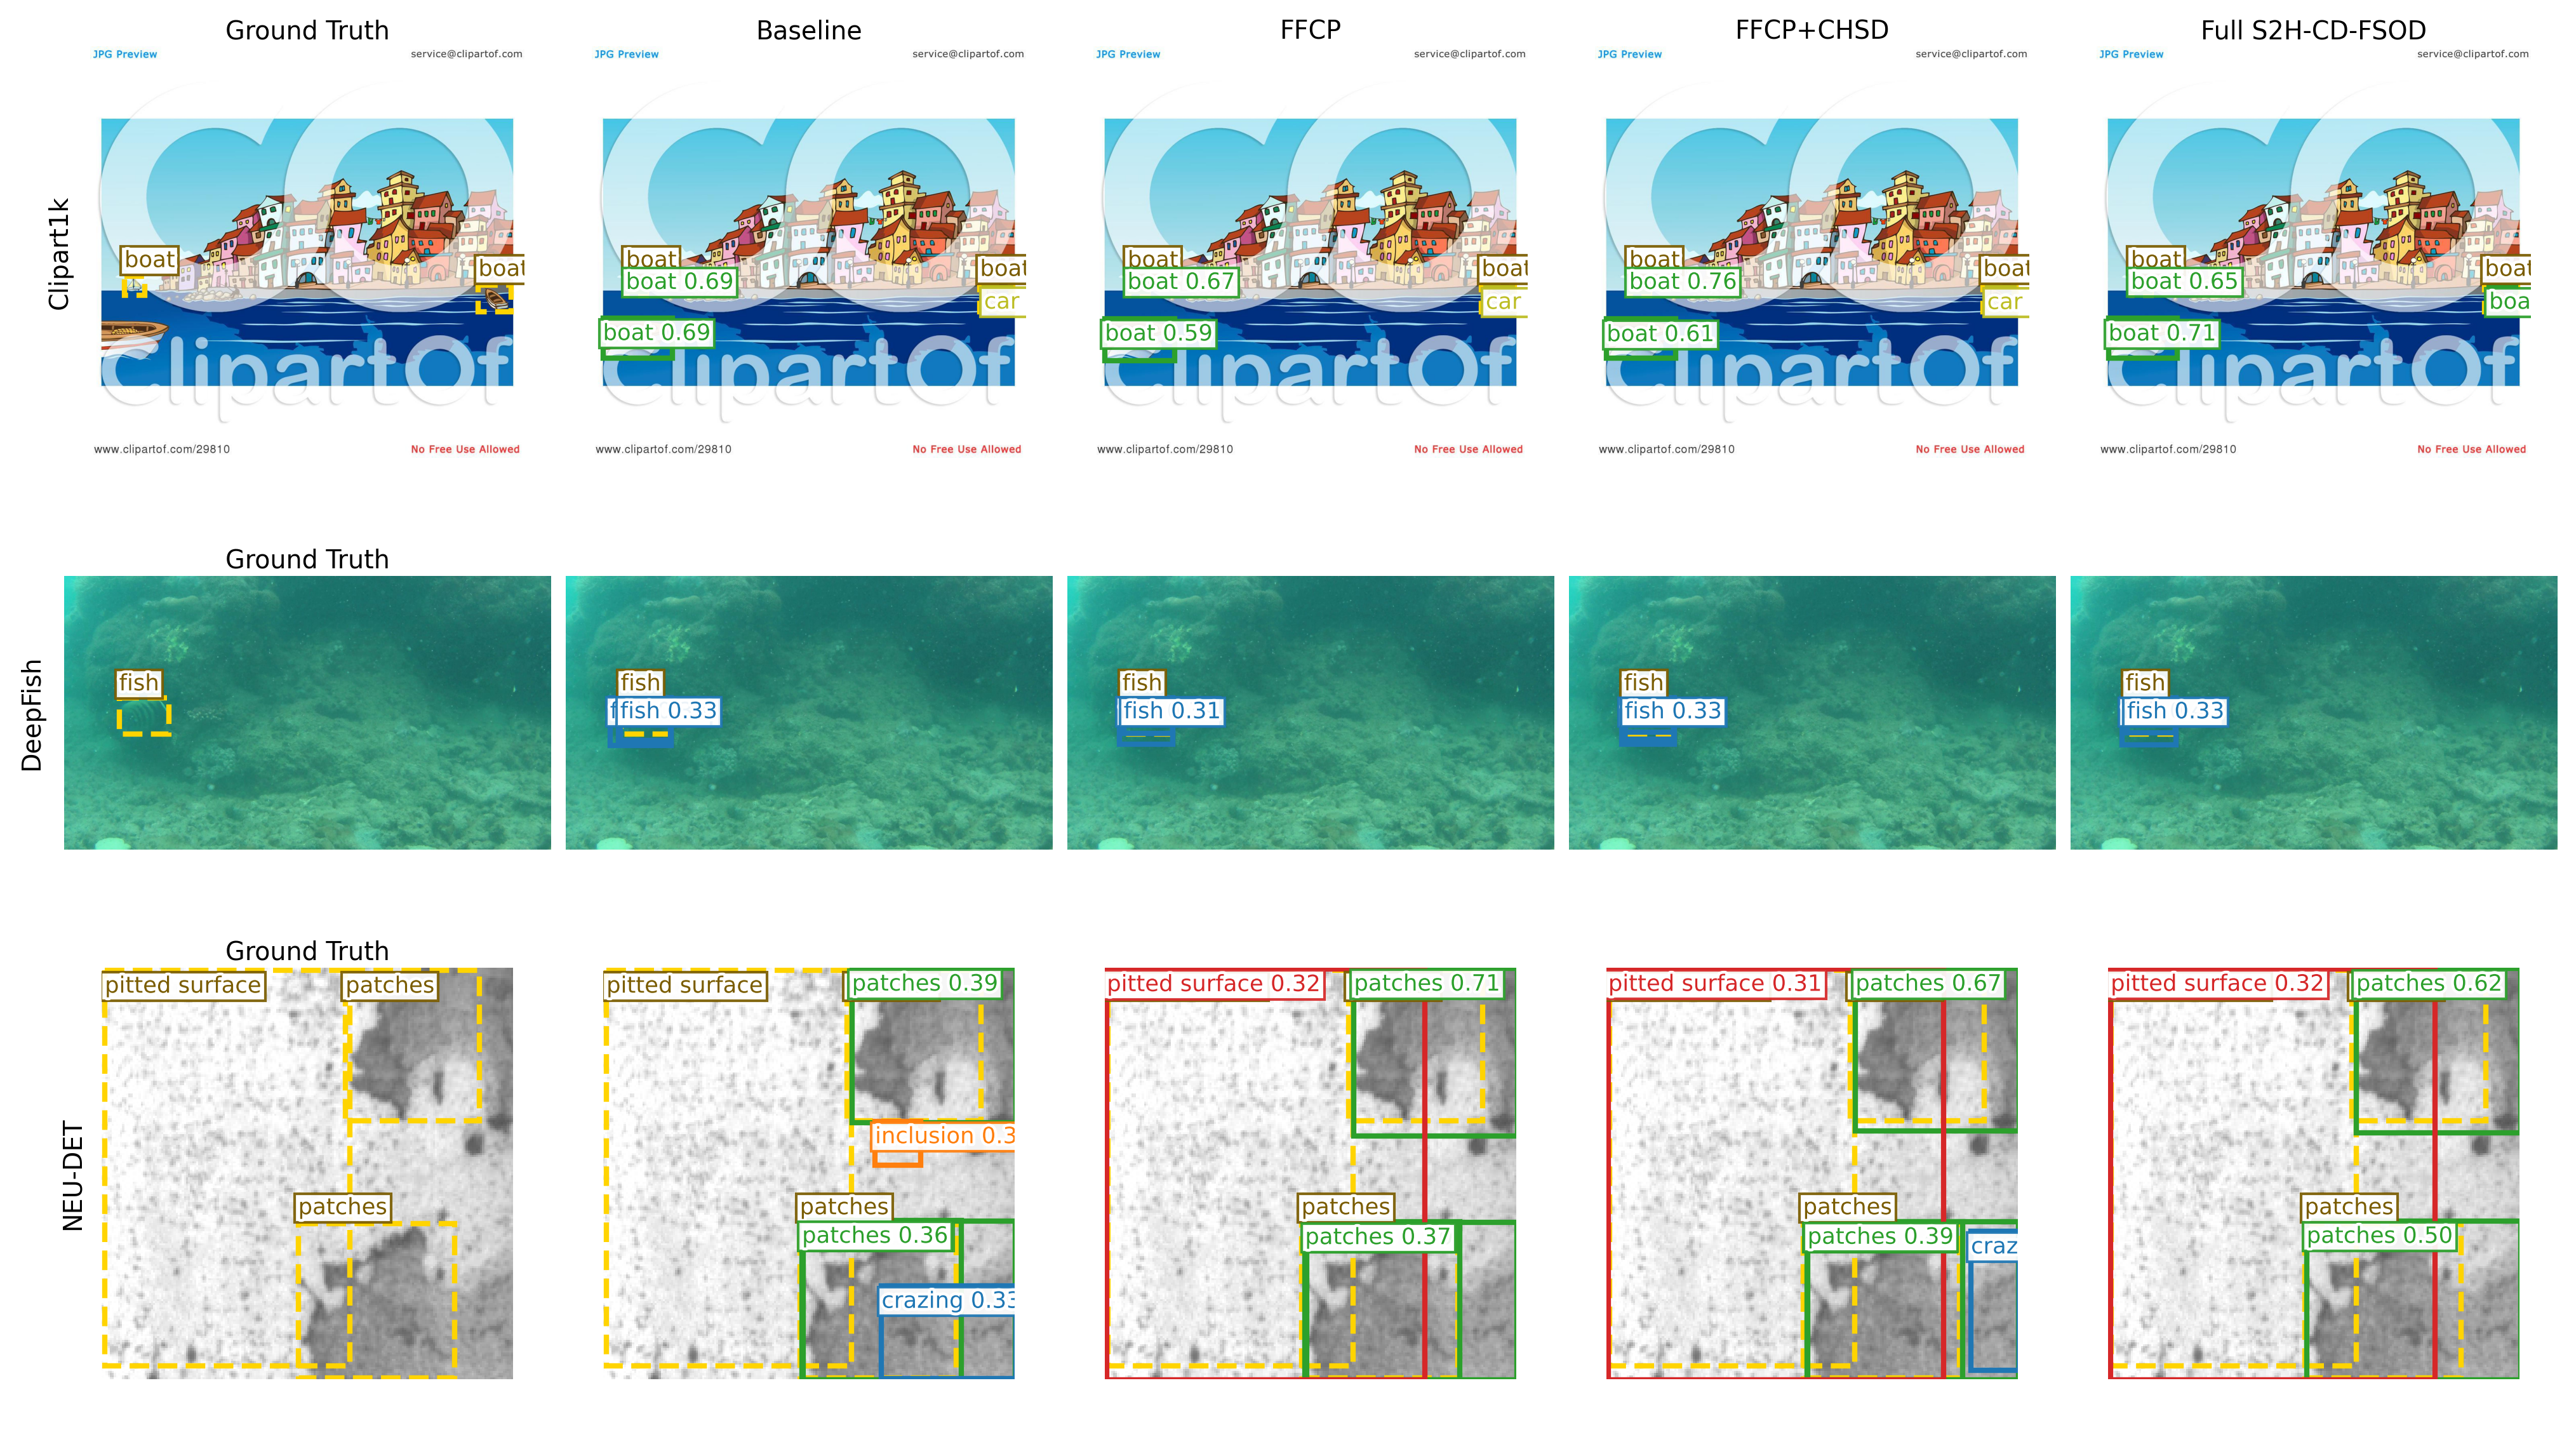
\includegraphics[width=\textwidth]{fig/confidence_progression.png}
    \caption{\textbf{Qualitative detection comparison on 5-shot target domains.}
    Each row shows a representative example from Clipart1k, DeepFish, and
    NEU-DET, while the columns progress from ground truth to the Grounding DINO
    baseline, FFCP, FFCP+CHSD, and the full S2H-CD-FSOD model. Yellow dashed
    boxes indicate annotated objects; colored prediction boxes are labeled with
    the predicted category and confidence score. The examples illustrate how the
    cumulative stages suppress context-driven or spurious responses while
    retaining detections of the target objects, with the largest changes
    occurring in the cluttered underwater and industrial scenes.}
    \label{fig:confidence_progression}
\end{figure*}
